\documentclass[tikz,border=8pt]{standalone}
% Shared look for every TikZ diagram. Load with \input{../../tools/tikz-style.tex}
\usepackage[sfdefault]{roboto}
\usetikzlibrary{arrows.meta, positioning, shapes.geometric, calc, fit, backgrounds}
\definecolor{cblue}{HTML}{4C78A8}
\definecolor{corange}{HTML}{F58518}
\definecolor{cgreen}{HTML}{54A24B}
\definecolor{cred}{HTML}{E45756}
\definecolor{cpurple}{HTML}{B279A2}
\definecolor{cgrey}{HTML}{6B6B6B}
\tikzset{
  every picture/.style={font=\sffamily, line width=1.2pt},
  box/.style={draw=#1, fill=#1!12, rounded corners=4pt, align=center, inner sep=7pt, minimum height=1.1cm},
  box/.default=cgrey,
  arrow/.style={-{Stealth[length=3mm]}, draw=cgrey, line width=1.4pt},
  title/.style={font=\sffamily\bfseries\Large},
  note/.style={font=\sffamily\small, text=cgrey, align=center},
}
\AtBeginDocument{\hyphenpenalty=10000 \exhyphenpenalty=10000}

% PX4's attitude autotuner (src/modules/mc_autotune_attitude_control): it shakes the drone with a train of steps, fits a
% model of the angular-rate dynamics with a second-order denominator, and computes PID gains for a requested
% closed-loop rise time (MC_AT_RISE_TIME, default 0.14 s; 0.2 s for yaw) with damping index 0, which
% pid_design.hpp documents as "0 is critical damping, 1 is Butterworth".
\begin{document}
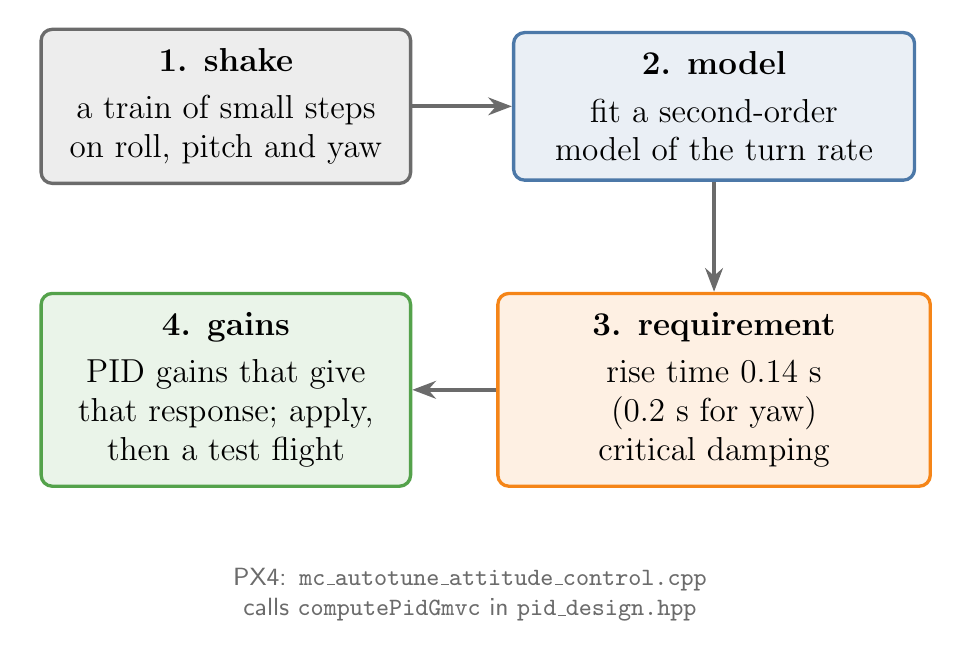
\begin{tikzpicture}[every node/.append style={font=\large}]
  \node[box=cgrey, text width=4.2cm] (test) at (0,0) {\textbf{1. shake}\\[3pt] a train of small steps\\ on roll, pitch and yaw};
  \node[box=cblue, text width=4.6cm] (model) at (6.2,0) {\textbf{2. model}\\[3pt] fit a second-order\\ model of the turn rate};
  \node[box=corange, text width=5.0cm] (spec) at (6.2,-3.6) {\textbf{3. requirement}\\[3pt] rise time 0.14 s\\ (0.2 s for yaw)\\ critical damping};
  \node[box=cgreen, text width=4.2cm] (gains) at (0,-3.6) {\textbf{4. gains}\\[3pt] PID gains that give\\ that response; apply,\\ then a test flight};
  \draw[arrow] (test) -- (model);
  \draw[arrow] (model) -- (spec);
  \draw[arrow] (spec) -- (gains);
  \node[note, text width=11cm] at (3.1,-6.2) {PX4: \texttt{mc\_autotune\_attitude\_control.cpp} calls \texttt{computePidGmvc} in \texttt{pid\_design.hpp}};
\end{tikzpicture}
\end{document}
